\documentclass{article}
\usepackage[utf8]{inputenc}


% This template is an adaptation from Christian Garbin's mtemplate:
% https://www.overleaf.com/latex/templates/model-card-template/fjmvzbbbxmwx
% Licensed under Creative Commons CC BY 4.0

% Few changes were made: table formatting, and removal of the explanation section.
% The intention behind these changes is for ease of use.

% For more information on Model Cards, please read the following article:
% https://arxiv.org/abs/1810.03993


\usepackage{setspace}
\usepackage{subcaption}
\usepackage{changepage} % to adjust margins
\usepackage[breakable]{tcolorbox}
\usepackage{float} % for tables inside tcolorbox https://tex.stackexchange.com/a/274342
\usepackage{enumitem}
\usepackage{geometry}

\geometry{vmargin=30pt,hmargin=30pt}
\begin{document}


% Each section is supposed to be brief, in the form of a bullet list.
% This environment formats the lists in each model card section in a compact format to help
% the card fit into the recommended "one to two pages".
\newenvironment{mcsection}[1]
    {%
        \textbf{#1}

        \begin{itemize}[leftmargin=*,topsep=0pt,itemsep=-1ex,partopsep=1ex,parsep=1ex,after=\vspace{\medskipamount}]
    }
    {%
        \end{itemize}
    }

\begin{singlespace}

\tcbset{colback=white!10!white}

% TITLE, change here
\begin{tcolorbox}[title=\textbf{Model Card},
    breakable, sharp corners, boxrule=0.7pt]

% Change to a smaller, but still legible font size.
\small{


\begin{mcsection}{Model Details}
    \item This model was developed by [INSTITUTION ANONYMIZED], 27/02/2026.
    \item Forecasting model, predicting the total hospitalizations by respiratory diseases for a given hospital and month.
    \item For comparison purposes, 4 models were implemented: a baseline (Linear Regression, with "scikit-learn"), LightGBM (model by Microsoft), LightGBM with leakage, and LightGBM after resampling.
\end{mcsection}

\begin{mcsection}{Intended Use}
    \item This model may be used by hospitals to help estimate how many hospitalizations should be expected for the following month, assisting them in other decisions derived from the prediction.
    \item This model can not be used for assistance on individual cases (patients).
\end{mcsection}

\begin{mcsection}{Factors}
    \item During data processing, hospitals with low monthly average for hospitalizations were filtered out. Therefore, this model is not recommended for use by smaller hospitals.
\end{mcsection}


\begin{mcsection}{Training Data}
    \item All data come from DataSUS. Specifically, from 2022 to 06/2024. Used files were the reduced version (RD) from the SIH portal.
    \item Pre-processing: all data was aggregated by hospital and month/year, calculating total counts, means, ratios and percentiles of some variables. Most data refers to information of previous months, with a few pointing to current (for leakage study).
    \item Hospitals with a monthly average lower then 5 hospitalizations were removed for robustness.
    \item Read \textit{data\_card.pdf} for more detailed information on the dataset and the pre-processing.
\end{mcsection}

\begin{mcsection}{Evaluation Data}
    \item For LightGBM, an extra dataset was used for validation (data from 07/2024 to 12/2024). It went through the same pre-processing as the training data.
    \item For evaluation, data from 2025 was used, which also went through the same pre-processing. (Note: December and data from November for "AC" and "RR" were not available during development)
\end{mcsection}

\begin{mcsection}{Métricas}
    \item Mean Absolute Error (MAE): metric for overall error analysis, without penalizing any kind of error. High MAE indicates high amount of errors or large errors.
    \item Root Mean Squared Error (RMSE): metric for overall error analysis, penalizing large errors. High RMSE indicates a high amount of larger errors.
    \item Symetric Mean Absolute Percentage Error (SMAPE): metric for percentage based error analysis. High SMAPE indicates a higher capacity for the prediction to be further from the real value.
\end{mcsection}

\begin{mcsection}{Ethical Considerations}
    \item A fairness study showed some disparity in prediction quality between some sensitives groups (mainly regional and hospital size). For more information, read \textit{fairness\_report.pdf}.
\end{mcsection}

\begin{mcsection}{Caveats and Recommendations}
    \item This model was developed for educational purposes. It's not meant to be used in real, professional environment.
\end{mcsection}

\pagebreak

\centering
\textbf{}
\begin{mcsection}{Quantitative Analyses}
    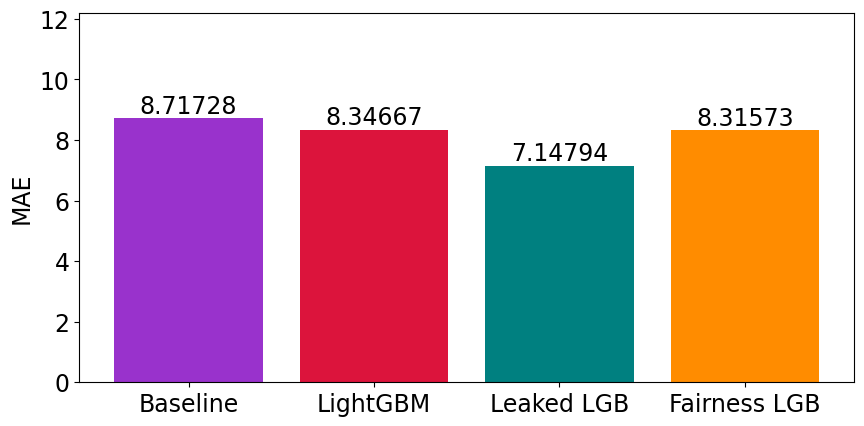
\includegraphics[width=0.3\linewidth]{../metric_Images/mae_general.png}
    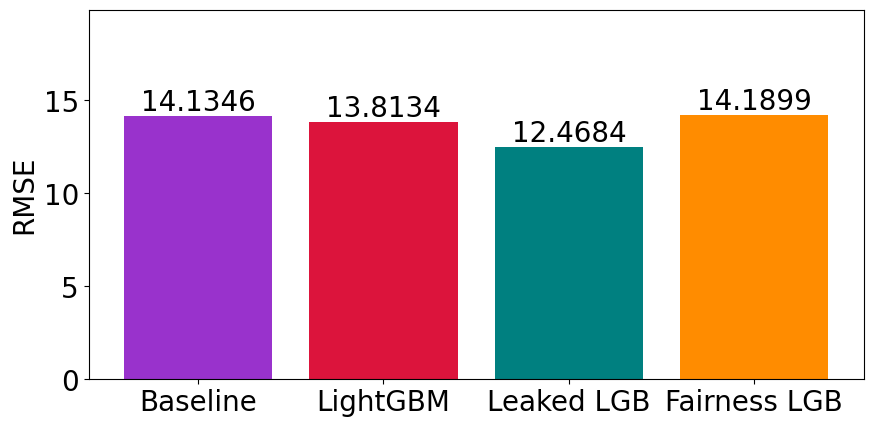
\includegraphics[width=0.3\linewidth]{../metric_Images/rmse_general.png}
    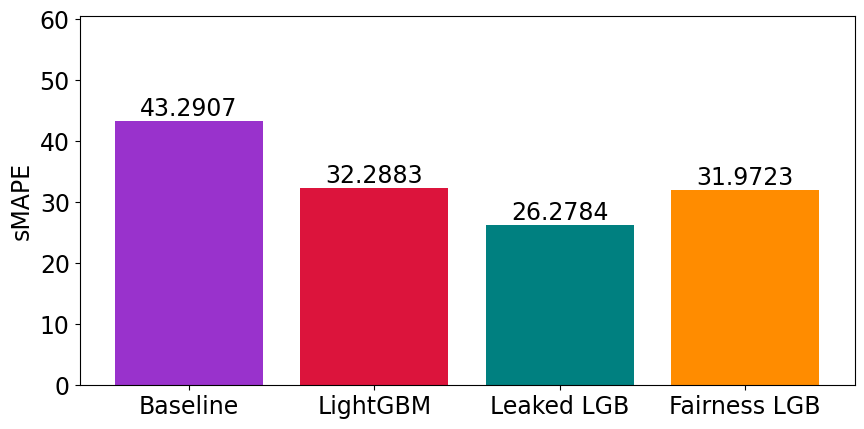
\includegraphics[width=0.3\linewidth]{../metric_Images/smape_general.png}
\end{mcsection}

}
\end{tcolorbox}
\end{singlespace}

\end{document}
